\begin{abstract}
%----Image Teaser----%
\begin{figure}[!h]
    \begin{center}
        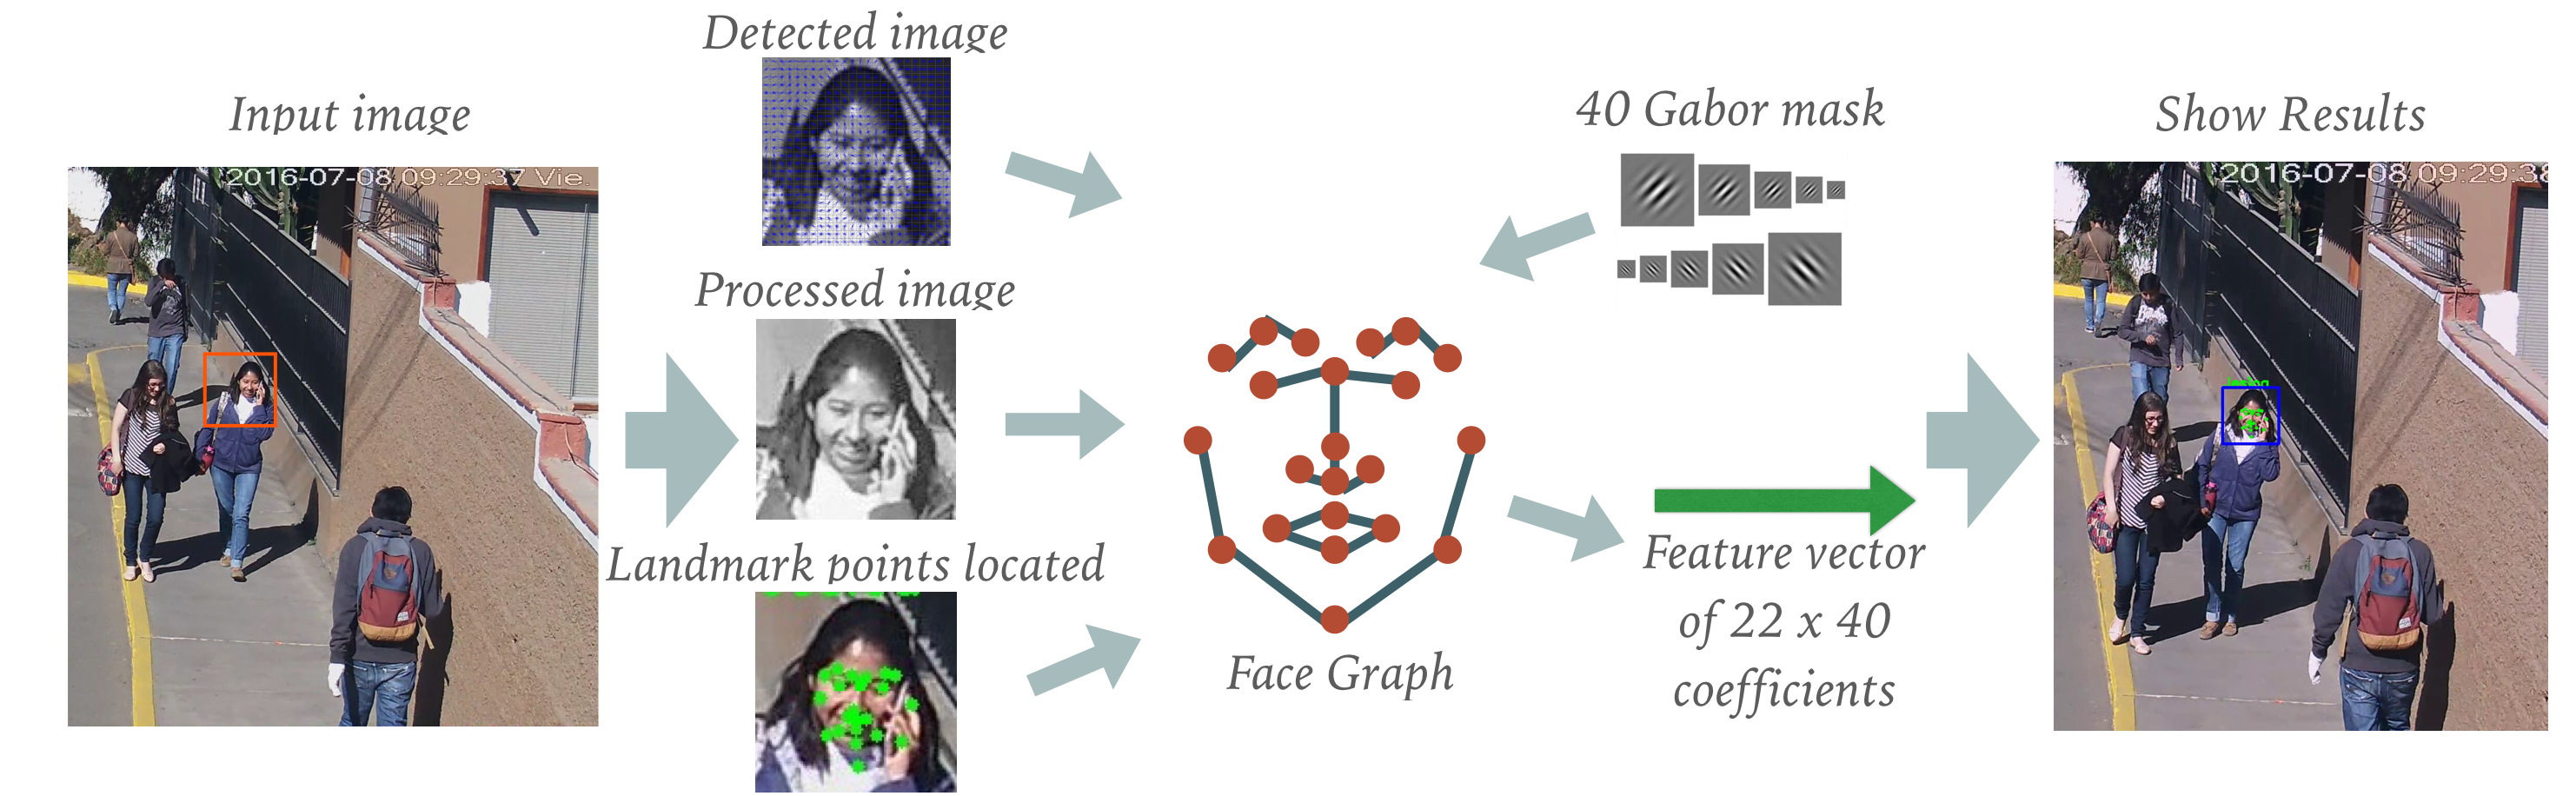
\includegraphics[width=\textwidth]{teaser.png}
    \end{center}
\end{figure}

Face recognition is an area with a large number of applications and techniques.
Many of these techniques provide good results when they are applied to situations where the environment in which recognition is desired is controlled, this is understood as the control of the factors that influence the recognition process, such as illumination, face pose , facial expression, etc.

But for the case of uncontrolled environments, such as video surveillance, face recognition still presents difficulties: variation in illumination, lack of collaboration of people to recognize, among several others.
Because of the importance it has in security and the amount of existing infrastructure, it is necessary to apply face recognition to video surveillance.

In this thesis, we propose a face recognition pipeline using \ac{EBGM} with \ac{CLNF} as a replacement for the point detection function of the original algorithm to finally be applied in video.

In addition we perform a parametric analysis of \ac{EBGM} to find the most influential factor in its performance along with its comparison with other methods of face recognition. we also determinate the elements that are part of the pipeline presented as final result.

Finally, we tested the proposal in a database we created from a security camera, consisting of 24 subjects with 8 images each. The final results show an improvement in images taken in the morning and at noon respectively.

\begin{flushleft}
\textbf{Keywords:} Face recognition, Video surveillance, Uncontrolled environment, \acf{EBGM}.
\end{flushleft}

\end{abstract}